\section{Multiple-Access Channel}
In the case of a multiple-access channel, two or more senders send information to a common receiver. A bunch of cell phones communicating with a base station is a prominent example of this channel. But in this case, senders face the receiver noise and interference from other senders.
%
\subsection{Some Definitions}
%
\begin{tcolorbox}[boxrule=0pt,frame hidden,sharp corners,enhanced, opacityback=0, borderline west={2pt}{0pt}{red}]
\begin{defn} \textbf{(Multiple-Access Channel)} A discrete memoryless multiple-access channel consists of three alphabets, $\mathcal{X}_1, \mathcal{X}_2,$ and $\mathcal{Y}$, and a probability transition matrix $p(y|x_1,x_2)$.
\end{defn}
\end{tcolorbox}
%
Now let us define a code corresponding to the multiple-access channel.
%
\begin{tcolorbox}[boxrule=0pt,frame hidden,sharp corners,enhanced, opacityback=0, borderline west={2pt}{0pt}{red}]
\begin{defn} \textbf{(A $((2^{nR_1},2^{nR_2}),n)$ code)} A $((2^{nR_1},2^{nR_2}),n)$ code for the multiple-access channel consists of two sets of integers $\mathcal{W}_1 = \{1,2,...,2^{nR_1}$ and $\mathcal{W}_2 = \{1,2,...,2^{nR_2}$, called the message sets, two encoding functions,
%
\begin{eqnarray}
    X_1: \mathcal{W}_1 \rightarrow \mathcal{X}_1^n,
\end{eqnarray}
%
and
%
\begin{eqnarray}
    X_2: \mathcal{W}_2 \rightarrow \mathcal{X}_2^n,
\end{eqnarray}
%
and a decoding function
\begin{eqnarray}
    g: \mathcal{Y}^n \rightarrow \mathcal{W}_1 \times \mathcal{W}_2.
\end{eqnarray}
%
\end{defn}
\end{tcolorbox}
%
As shown in the diagram, there are two senders and one receiver for this channel. Sender 1 (Sender 2) chooses an index $W_1$ uniformly from the set $\{1,2,...,2^{nR_1}\}$ ($\{1,2,...,2^{nR_2}\}$) and sends the codeword over the channel. Let us assume that the messages are independent and equally likely. In other words, the distribution of messages over the product set $\mathcal{W}_1 \times \mathcal{W}_2$ is uniform. In that case, we can define the average probability of error.
%
\begin{tcolorbox}[boxrule=0pt,frame hidden,sharp corners,enhanced, opacityback=0, borderline west={2pt}{0pt}{red}]
\begin{defn} \textbf{(Average Probability of error)} The average probability of error for the $((2^{nR_1},2^{nR_2}),n)$ code is given by
%
\begin{eqnarray}
    P_e^{(n)} = \frac{1}{2^{n(R_1+R_2)}} \sum_{(w_1,w_2)\in \mathcal{W}_1 \times \mathcal{W}_2}\Pr {g(Y^n) \neq (w_1, w_2)|(w_1, w_2) \quad \text{sent}}.
\end{eqnarray}
\end{defn}
\end{tcolorbox}
%
%
\begin{tcolorbox}[boxrule=0pt,frame hidden,sharp corners,enhanced, opacityback=0, borderline west={2pt}{0pt}{red}]
\begin{defn} \textbf{(Achievable rate pair)} A rate pair $(R_1, R_2)$ is said to be achievable for the multiple-access channel if there exists a sequence of $((2^{nR_1},2^{nR_2}),n)$ codes with $P_e^{(n)}\rightarrow 0$.
\end{defn}
\end{tcolorbox}
%
Now, let us define the capacity region.
%
\begin{tcolorbox}[boxrule=0pt,frame hidden,sharp corners,enhanced, opacityback=0, borderline west={2pt}{0pt}{red}]
\begin{defn} \textbf{(The capacity region)} The capacity region of the multiple-access channel is the closure of the set of achievable $(R_1, R_2)$ rate pairs.
\end{defn}
\end{tcolorbox}
%
But it is better understood via the theorem.
%%%%%%%%%%%%%%%%%%%%%%%%%%%%%%%%%%%%%%%%%%%%%%%%%%%%%%%%%%%%%%
\subsection{Multiple-access channel capacity and Some examples}
%
\begin{tcolorbox}[boxrule=0pt,frame hidden,sharp corners,enhanced, opacityback=0, borderline west={2pt}{0pt}{blue}]
\begin{thm} The capacity of a multiple-access channel $(\mathcal{X}_1 \times \mathcal{X}_2, p(y|x_1,x_2), \mathcal{Y})$ is the closure of the convex hull of all $(R_1, R_2)$ satisfying
%
\begin{eqnarray}
    R_1 &<& I(X_1; Y|X_2); \\
    R_2 &<& I(X_2; Y|X_1); \\
    R_1+R_2 &<& I(X_1, X_2; Y) \label{8.2.1}
\end{eqnarray}
%
for some product distribution $p(x_1)p(x_2)$ on $\mathcal{X}_1 \times \mathcal{X}_2$.
\end{thm}
\end{tcolorbox}
%

\subsection{Different Capacity region for the Multiple-Access Channel}
For a distribution of $p_1(x_1)p_2(x_2)$, the capacity region is shown in figure \ref{fig:MAC}.\\
%
\begin{figure}[h]
    \centering
    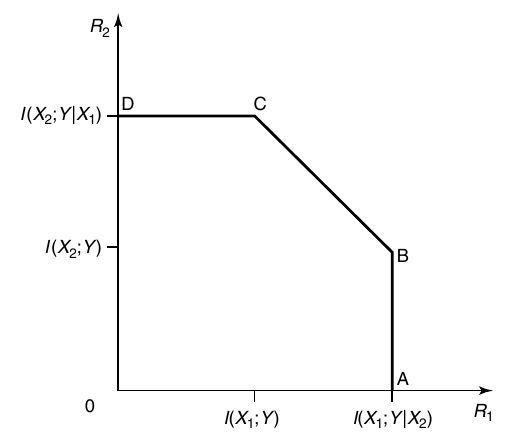
\includegraphics[scale=0.35]{Diagrams/Achievable region of MAC.png}
    \caption{Achievable region of multiple-access channel for a fixed input distribution}
    \label{fig:MAC}
\end{figure}
%
\linebreak There are 4 corner points in this diagram. Let us discuss briefly each and every point. 
%
\begin{enumerate}
    \item \textbf{Point A:} In this case, sender 2 is not sending any information. Therefore, the maximum rate is achievable due to sender 1. Therefore for any distribution $p_1(x_1)p_2(x_2)$,
    %
    \begin{eqnarray}
        I(X_1;Y|X_2) &=& \sum_{x_2} p_2(x_2)I(X_1;Y|X_2=x_2) \\
        &\leq& \max_{x_2}  I(X_1;Y|X_2=x_2).
    \end{eqnarray}
    %
    This is because the average is less than the maximum. Therefore,
    %
    \begin{eqnarray}
        \max R_1 = \max_{p_1(x_1)p_2(x_2)}  I(X_1;Y|X_2)= \max_{x_2}  I(X_1;Y|X_2=x_2),
    \end{eqnarray}
    %
    \textit{i.e.}, maximum is attained when we set $X_2 = x_2$.

    \item \textbf{Point B:} This point suggests the maximum rate at which sender 2 can send as long as sender 1 sends at his/her maximum rate. If $X_1$ is regarded as noise for the channel from $X_2$ to $Y$, this is the rate that is achieved. With the help of single-user channel results, $X_2$ can transmit at a rate of $I(X_2; Y)$. The receiver definitely knows about the $X_2$ codeword, and he/she can subtract its effect from the channel. The average mutual information, where the average is across these channels, and each channel occurs as many times as the correct $X_2$ symbol appears in the codewords, is the $X_1$ rate that is attained in this instance. Therefore, the obtained rate is
    %
    \begin{eqnarray}
        \sum_{x_2} p(x_2)I(X_1;Y|X_2 = x_2) = I(X_1;Y|X_2).
    \end{eqnarray}

    \item \textbf{Point C:} This point corresponds to point B, where the receiver and sender roles are interchanged.

    \item \textbf{Point D:} This point corresponds to point A, where the receiver and sender roles are interchanged.
\end{enumerate}
%
The other points can be achieved by time-sharing\footnote{A multiple access approach called time-division multiple access (TDMA) divides a communication resource into time slots so that numerous users can share it.}. Thus, we can interpret the capacity region of a multiple-access channel as a single-user interpretation.
%%%%%%%%%%%%%%%%%%%%%%%%%%%%%%%%%%%%%%%%%%%
\subsection{Convexity of the Capacity Region of the Multiple-Access Channel and Its Consequences}
In this subsection, we will state some theorems and lemmas. 
%
\begin{tcolorbox}[boxrule=0pt,frame hidden,sharp corners,enhanced, opacityback=0, borderline west={2pt}{0pt}{blue}]
\begin{thm} 
The capacity region $\mathcal{C}$ of a multiple-access channel is convex [i.e., if $(R_1,R_2) \in \mathcal{C}$ and $(R'_1,R'_2) \in \mathcal{C}$, then $(\lambda R_1+(1-\lambda)R'_1, \lambda R_2+(1-\lambda)R'_2) \in \mathcal{C}$ for $0 \leq \lambda \leq 1$].
\end{thm}
\end{tcolorbox}
%
In the case of the pentagonal region as shown in figure \ref{fig:MAC}, the capacity region for a fixed $p(x_1)p(x_2)$ is defined by three mutual informations, $I_1 = I(X_1;Y|X_2), I_2 = I(X_2;Y|X_1)$, and $I_1 = I(X_1, X_2; Y)$. Therefore, we can define a rate region
%
\begin{eqnarray}
    C_{\mathbf{I}} = \{ (R_1, R_2): R_1\geq 0, R_2 \geq 0, R_2 \leq I_1, R_2 \leq I_2, R_1+R_2 \leq I_3 \}.
    \label{6.4.1}
\end{eqnarray}
%
There is an additional property with the theorem.
%
\begin{eqnarray}
    I(X_2;Y|X_1) &=& H(X_2|X_1)-H(X_2|Y,X_1) \nonumber\\
    &=& H(X_2)-H(X_2|Y,X_1) \nonumber\\
    &=& I(X_2;Y,X_1) \nonumber\\
    &=& I(X_2;Y) + I(X_2;X_1|Y) \nonumber\\
    &\geq& I(X_2;Y) 
\end{eqnarray}
%
Therefore we can write
%
\begin{eqnarray}
    I(X_1;Y|X_2)+I(X_2;Y|X_1) &\geq& I(X_1;Y|X_2)+I(X_2;Y) \nonumber\\
    &=& I(X_1,X_2;Y)
\end{eqnarray}
%
So,
%
\begin{eqnarray}
    I_1+I_2 \geq I_3.
\end{eqnarray}
%
\begin{tcolorbox}[boxrule=0pt,frame hidden,sharp corners,enhanced, opacityback=0, borderline west={2pt}{0pt}{green}]
\begin{lemma} 
Let $\mathbf{I}_1, \mathbf{I}_2 \in \mathcal{R}^3$ be two vectors of mutual informations that define rate refions $C_{\mathbf{I}_1}$ and $C_{\mathbf{I}_2}$, respectively, as given in \eqref{6.4.1}. For $0\leq \lambda \leq 1$, define $\mathbf{I}_\lambda = \lambda\mathbf{I}_1+(1-\lambda)\mathbf{I}_2$, and let $C_{\mathbf{I}_\lambda}$ be the rate region defined by $\mathbf{I}_\lambda$. Then
%
\begin{eqnarray}
    C_{\mathbf{I}_\lambda} = \lambda C_{\mathbf{I}_1}+(1-\lambda)C_{\mathbf{I}_2}.
\end{eqnarray}
\end{lemma}
\end{tcolorbox}
%
The immediate consequence of this lemma is the following theorem:
%
\begin{tcolorbox}[boxrule=0pt,frame hidden,sharp corners,enhanced, opacityback=0, borderline west={2pt}{0pt}{blue}]
\begin{thm} 
The convex hull of the union of the rate regions defined by individual $\mathbf{I}$ vectors equals the rate region defined by the convex hull of the $\mathbf{I}$ vectors.
\end{thm}
\end{tcolorbox}
%
This concept on the equivalence of the convex hull operation on the rate regions with the convex combinations of the mutual information can be mapped to the general $m$-user multiple-access channel.
%
\begin{tcolorbox}[boxrule=0pt,frame hidden,sharp corners,enhanced, opacityback=0, borderline west={2pt}{0pt}{blue}]
\begin{thm} 
\textbf{(Multiple-Access Channel)}
\begin{enumerate}
    \item The set of achievable rates of a discrete memoryless multiple-access channel is given by the closure of the set of all $(R_1, R_2)$ pairs satisfying
%
\begin{eqnarray}
    R_1 &<& I(X_1;Y|X_2,Q), \nonumber\\
    R_2 &<& I(X_2;Y|X_1,Q), \nonumber\\
    R_1+R_2 &<& I(X_1,X_2;Y|Q)
\end{eqnarray}
%
for some choice of the joint distribution $p(q)p(x_1|q)p(x_2|q)p(y|x_1,x_2)$ with $\abs{\mathcal{Q}}\leq 4$.

\item (Converse) Given any sequence of $((2^{nR_1},2^{nR_2}),n)$ codes with $P_e^{(n)} \rightarrow 0$, the rates must satisfy 

\begin{eqnarray}
    R_1 &<& I(X_1;Y|X_2,Q), \nonumber\\
    R_2 &<& I(X_2;Y|X_1,Q), \nonumber\\
    R_1+R_2 &<& I(X_1,X_2;Y|Q)
    \label{8.4.1}
\end{eqnarray}
%
for some choice of random variable $Q$ defined on $\{1,2,3,4 \}$ and joint distribution $p(q)p(x_1|q)p(x_2|q)p(y|x_1,x_2)$.
\end{enumerate}

\end{thm}
\end{tcolorbox}
%
By proving this theorem, we can show that every point in the region defined by \eqref{8.4.1} is achievable. In the converse case, it can be shown that the region in \eqref{8.4.1} was the best that can be done, and this is the capacity region of the channel too. Finally, the region in \eqref{8.2.1} cannot be any larger than the region in \eqref{8.4.1}. This is the capacity region of the multiple-access channel. 
%%%%%%%%%%%%%%%%%%%%%%%%%%%%%%%%%%%%%%%%%%%%%%%%%

\subsection{$m$-User Multiple-Access Channels}
It is possible to generalize the result derived in the previous subsections for two senders to $m$ senders where $m\geq 2$. A multiple-access channel is shown in the figure \ref{fig:m-MAC}. Here the sender $1,2,...,m$ sends the independent indices $w_1,w_2,...,w_m$ over the channel respectively. As this is nothing but the extension of a two-sender case, the codes, rates, and achievability are all defined in exactly the same way.\\
%
\begin{figure}[h]
    \centering
    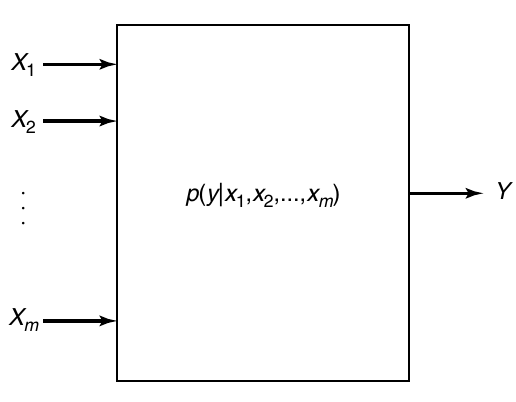
\includegraphics[scale=0.30]{Diagrams/M-user MAC.png}
    \caption{$m$-user Multiple-access channel}
    \label{fig:m-MAC}
\end{figure}
%
\linebreak Here, we have the following theorem.
%
\begin{tcolorbox}[boxrule=0pt,frame hidden,sharp corners,enhanced, opacityback=0, borderline west={2pt}{0pt}{blue}]
\begin{thm} 
Let $S \subseteq \{1,2,...,m\}$ and $S^c$ denote the complement of $S$. Let $R(S)=\sum_{i \in S} R_i$, and let $X(S)=\{X_i: I \in S$. Then, the capacity region of the $m$-user multiple-access channel is the closure of the convex hull of the rate vectors satisfying
%
\begin{eqnarray}
    R(S) \leq I(X(S);Y|X(S^c)) \quad \text{for all } S \subset \{1,2,...,m\}
\end{eqnarray}
%
for some product distribution $p_1(x_1)p_2(x_2)...p_m(x_m)$.
\end{thm}
\end{tcolorbox}
%